
\documentclass[10pt]{article}
\usepackage[a4paper,left=1.7cm,right=1.7cm,top=2.3cm,bottom=2.3cm,headheight=0.9cm,headsep=0.35cm,footskip=1.0cm]{geometry}
\usepackage{amsmath,amssymb,mathtools}
\usepackage{xcolor,graphicx,array,booktabs,enumitem,lastpage,pgffor}
\usepackage{tikz}
\usetikzlibrary{arrows.meta,calc,patterns}
\usepackage[most]{tcolorbox}
\usepackage{fancyhdr}
\usepackage{fontspec}\usepackage{microtype}
\definecolor{NAVY}{HTML}{1F3A5F}\definecolor{INK}{HTML}{1A1A1A}\definecolor{TEAL}{HTML}{1A7F8E}
\definecolor{BLUE}{HTML}{2F6DB5}\definecolor{ORANGE}{HTML}{E07B39}\definecolor{GREY}{HTML}{6B7280}
\definecolor{GOLD}{HTML}{C9A227}\definecolor{LINE}{HTML}{C7CDD6}
\setlength{\parindent}{0pt}\setlength{\parskip}{3pt}
\renewcommand{\arraystretch}{1.25}
\newcommand{\WSCODE}{SAT-M \textperiodcentered\ W1-B}
\pagestyle{fancy}\fancyhf{}
\renewcommand{\headrulewidth}{0.5pt}\renewcommand{\headrule}{\hbox to\headwidth{\color{NAVY}\leaders\hrule height \headrulewidth\hfill}}
\renewcommand{\footrulewidth}{0pt}
\fancyhead[L]{\small\bfseries\color{NAVY}SAT Math Mastery \textperiodcentered\ Week 1 \textperiodcentered\ Session B \textemdash\ Lines, Slope \& Linear Functions}
\fancyhead[R]{\small\color{GREY}Mr Malek Thiab}
\fancyfoot[L]{\footnotesize\color{GREY}\WSCODE}
\fancyfoot[C]{\footnotesize\color{NAVY}{\addfontfeatures{LetterSpace=18}\textsc{Faith, Righteousness and Wisdom}}}
\fancyfoot[R]{\footnotesize\color{GREY}Mr Malek Thiab \textperiodcentered\ Page \thepage\ of \pageref{LastPage}}
\newtcolorbox{cbox}[2][]{enhanced,breakable,colback=#2!5,colframe=#2!70!black,boxrule=0.6pt,arc=2pt,left=5pt,right=5pt,top=3pt,bottom=3pt,fonttitle=\bfseries\small,#1}
\newcommand{\banner}[1]{\vspace{6pt}\par\noindent\begin{tcolorbox}[enhanced,colback=NAVY,colframe=NAVY,boxrule=0pt,arc=2pt,left=6pt,top=1pt,bottom=1pt,nobeforeafter]\color{white}\bfseries\small\MakeUppercase{#1}\end{tcolorbox}\par\nopagebreak\vspace{2pt}}
\newcommand{\worklines}[1]{\par\nopagebreak\foreach \i in {1,...,#1}{\par\vspace{0.74cm}{\color{LINE}\hrule height 0.4pt}}\par\vspace{4pt}}
\newcommand{\lvl}[1]{\textcolor{GREY}{\scriptsize\textsc{#1}}}
\newcommand{\choice}[4]{\par\vspace{2pt}\begin{tabular}{@{}p{0.47\linewidth}p{0.47\linewidth}@{}}(A)\ #1 & (B)\ #2\\ (C)\ #3 & (D)\ #4\end{tabular}}
\begin{document}


\begin{tcolorbox}[enhanced,colback=NAVY!4,colframe=NAVY,boxrule=0.8pt,arc=3pt]
{\Large\bfseries\color{NAVY} SAT Math Mastery Program \textperiodcentered\ Week 1, Session B}\\[2pt]
{\large\bfseries Lines, Slope \& Linear Functions}\\[3pt]
\begin{tabular}{@{}p{0.2\linewidth}p{0.75\linewidth}@{}}
\textbf{Time} & 120 minutes: 90 min solving \,+\, 30 min self-check and error log\\
\textbf{Target topics} & slope from points/graphs/tables \textperiodcentered\ forms of a line \textperiodcentered\ intercepts \textperiodcentered\ parallel \& perpendicular \textperiodcentered\ translations \textperiodcentered\ meaning of slope/intercept \textperiodcentered\ linear function notation\\
\textbf{Teacher} & Mr Malek Thiab \textperiodcentered\ Dar Alfikr School\\
\textbf{Name / Date} & \rule{5.5cm}{0.3pt}\ \ \rule{3cm}{0.3pt}\\
\end{tabular}
\end{tcolorbox}

\banner{1 \textperiodcentered\ Skills \& Ideas}
\begin{enumerate}[leftmargin=1.6em,itemsep=0pt,label=\textbf{S\arabic*.}]
\item Find slope from two points, a graph, a table, a standard-form equation, or a verbal rate.
\item Write and convert between slope-intercept, point-slope, standard and intercept forms.
\item Find $x$- and $y$-intercepts and use them (areas, conditions, context meaning).
\item Parallel and perpendicular lines, including directly from $Ax+By=C$.
\item Translate a line (up/down/left/right) and track slope and intercepts.
\item Interpret slope and intercept in context; build $f(x)=mx+b$ from data and solve for inputs.
\item Coordinate reasoning: collinearity, midpoint, perpendicular bisector, triangles cut by axes.
\item Parameter conditions on lines (a constant fixes slope, intercept, perpendicularity or area).
\end{enumerate}
\banner{2 \textperiodcentered\ Required Facts}
\begin{itemize}[leftmargin=1.4em,itemsep=0pt]
\item Slope $=\dfrac{\text{rise}}{\text{run}}=$ constant rate of change; the $y$-intercept is the value at $x=0$; the $x$-intercept is where $y=0$.
\item Horizontal line $y=c$: slope $0$. Vertical line $x=c$: slope undefined.
\item Parallel $\iff$ equal slopes (different intercepts). Perpendicular $\iff$ slopes are negative reciprocals (product $-1$).
\item A function is linear if equal steps in $x$ give equal steps in $y$ (check every gap in a table).
\item Shifting a graph up $k$ adds $k$ to $y$; slope never changes under a translation.
\item Two points determine a line; on a graph read only points that sit exactly on grid intersections.
\end{itemize}
\banner{3 \textperiodcentered\ Required Formulas}
\vspace{-4pt}\[
m=\dfrac{y_2-y_1}{x_2-x_1},\qquad y=mx+b,\qquad y-y_1=m(x-x_1),\qquad \dfrac xa+\dfrac yb=1
\]
\vspace{-8pt}\[
Ax+By=C:\ \ m=-\dfrac AB,\ \ \text{$x$-int }\dfrac CA,\ \ \text{$y$-int }\dfrac CB,\qquad \text{area with axes}=\dfrac12\left|\dfrac CA\cdot\dfrac CB\right|
\]
\vspace{-8pt}\[
\parallel:\ A_1B_2=A_2B_1,\qquad \perp:\ A_1A_2+B_1B_2=0,\qquad \text{midpoint}=\left(\dfrac{x_1+x_2}2,\dfrac{y_1+y_2}2\right),\qquad f(a+d)-f(a)=md
\]
\banner{4 \textperiodcentered\ Mini Theory Sheet}

\textbf{Choose the form by the data.}
\begin{center}\begin{tabular}{@{}ll@{}}\toprule
Given & Fastest route\\\midrule
two points & $m=\frac{\Delta y}{\Delta x}$, then point-slope with either point\\
slope and $y$-intercept & $y=mx+b$ directly\\
both intercepts $(a,0),(0,b)$ & $\frac xa+\frac yb=1$, or $m=-\frac ba$\\
$Ax+By=C$ & read $m=-\frac AB$; set $x=0$ or $y=0$ for intercepts\\
a table & $m$ from any two rows; confirm the rest have the same $m$\\\bottomrule\end{tabular}\end{center}

\textbf{Perpendicular in standard form.} Swap the coefficients and negate one: $\perp$ to $Ax+By=C$ is $Bx-Ay=C'$; find $C'$ from the given point.

\textbf{Parallel in standard form.} Keep $A,B$ (or scale both), change only $C$.

\textbf{Translation.} Down $k$: $b\to b-k$, and the $x$-intercept moves by $\frac km$. Same slope, always.

\textbf{Meaning.} In $y=mx+b$: $m$ = change in $y$ per $1$ unit of $x$; $b$ = starting value. Units of $m$ are (units of $y$)/(units of $x$).

\textbf{Constant conditions.} Turn the condition (slope, perpendicular, area, collinear) into one equation in the constant, then solve.

\textbf{Whole-number contexts.} Solve $f(x)=\text{target}$; if $x$ must be a whole day/trip/session, round to the first value that \emph{reaches} the target.
\begin{cbox}[title={5 \textperiodcentered\ Strategy Box}]{ORANGE}
\textbf{Shortcuts.} (1) Build slope as a fraction; never convert to a decimal until the end. (2) On a graph, use two lattice points far apart. (3) Verify any final equation by plugging both original points. (4) Perpendicular: swap and negate. (5) Intercept triangle: area $=\frac12|a||b|$, no integration of ideas needed.\\
\textbf{Traps.} $\frac{\Delta x}{\Delta y}$ inverted $\cdot$ sign lost in $y_2-y_1$ vs.\ $x_2-x_1$ order mismatch $\cdot$ reading the $y$-value of a point as the intercept $\cdot$ parallel vs.\ perpendicular confusion $\cdot$ ``what does the \emph{slope} mean'' answered with the intercept $\cdot$ forgetting the answer must be a whole day/trip.\\
\textbf{Calculator (Desmos).} Plot points as $(x,y)$, add \texttt{y\textasciitilde mx+b}, drag sliders to match; use a table to test integer inputs; type equations in standard form directly; click an intersection to read exact coordinates.\\
\textbf{Timing.} Easy $\le1.5$ min $\cdot$ Medium $\le3$ $\cdot$ Hard $\le4.5$ $\cdot$ Challenge $\le7$ (total $\approx80$ min).\\
\textbf{Pattern cues.} ``parallel'' $\to$ same $m$ $\cdot$ ``perpendicular'' $\to$ $-\frac1m$ $\cdot$ ``increases by \dots\ for every \dots'' $\to$ $m$ $\cdot$ ``bounded by the axes'' $\to$ intercepts $\cdot$ ``for all $a$: $f(a+d)-f(a)$'' $\to$ slope $\cdot$ ``first day/trip that \dots'' $\to$ round up.\end{cbox}
\banner{6 \textperiodcentered\ Guided Examples}
\begin{cbox}[title={Example 1 \textemdash\ Two points $\to$ equation $\to$ intercepts}]{TEAL}
A line passes through $(-1,7)$ and $(3,-1)$. Find its equation and both intercepts.\\[2pt]
$m=\dfrac{-1-7}{3-(-1)}=\dfrac{-8}{4}=-2$. Point-slope: $y-7=-2(x+1)\Rightarrow y=-2x+5$.\\
$y$-intercept $5$; $x$-intercept: $0=-2x+5\Rightarrow x=\frac52$. \emph{Check:} $(3,-1)$: $-6+5=-1$. \checkmark
\end{cbox}
\begin{cbox}[title={Example 2 \textemdash\ Perpendicular through a point (standard form)}]{TEAL}
Line $\ell$: $4x-3y=12$. Write the line through $(2,-1)$ perpendicular to $\ell$.\\[2pt]
Swap and negate: $3x+4y=C'$. Plug in $(2,-1)$: $C'=3(2)+4(-1)=2$. Answer: $3x+4y=2$.\\
\emph{Check:} $A_1A_2+B_1B_2=4\cdot3+(-3)(4)=0$. \checkmark
\end{cbox}
\begin{cbox}[title={Example 3 \textemdash\ Meaning of slope and intercept}]{TEAL}
A gym plan costs $340$ SAR after $2$ months and $640$ SAR after $5$ months (linear). Write $C(m)$ and interpret its parts.\\[2pt]
$\text{slope}=\dfrac{640-340}{5-2}=100$. $C(m)=100m+b$; $340=200+b\Rightarrow b=140$. So $C(m)=100m+140$.\\
$100$ = SAR per month; $140$ = joining fee (cost at $m=0$).
\end{cbox}
\newpage\banner{7 \textperiodcentered\ Practice Set \textemdash\ 24 problems \textperiodcentered\ Easy $\to$ Medium $\to$ Hard $\to$ SAT Challenge}
\small Write your work in the space below each problem. Circle your final answer. Multiple choice: one correct option. Student-produced response (SPR): enter an exact value (fraction or decimal).\normalsize\par\vspace{4pt}
\begin{minipage}{\linewidth}\textbf{\textcolor{NAVY}{1.}}\hfill\lvl{Easy \textperiodcentered\ No calculator needed}\\[1pt]What is the slope of the line in the $xy$-plane that passes through $(-2,5)$ and $(4,-7)$?\choice{$-2$}{$-\tfrac12$}{$\tfrac12$}{$2$}\worklines{4}\end{minipage}\par\vspace{2pt}

\begin{minipage}{\linewidth}\textbf{\textcolor{NAVY}{2.}}\hfill\lvl{Easy \textperiodcentered\ Desmos}\\[1pt]The graph of a line is shown in the $xy$-plane. Which equation represents the line?\begin{center}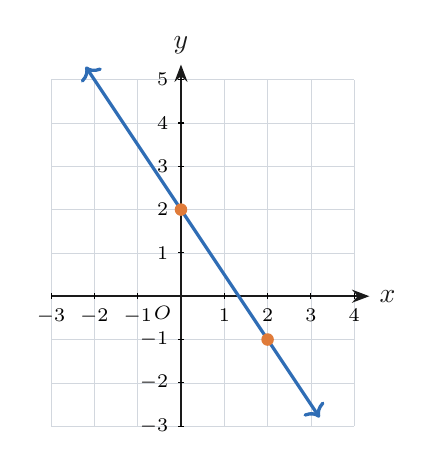
\begin{tikzpicture}[x=0.55cm,y=0.55cm,scale=1.0]
\tikzset{axisline/.style={-{Stealth[length=2.2mm]},thick,INK},gridl/.style={LINE!80,very thin},
 ln/.style={very thick,BLUE},pt/.style={circle,fill=ORANGE,inner sep=1.6pt}}
\draw[gridl] (-3,-3) grid[xstep=1,ystep=1] (4,5);
\draw[axisline] (-3,0) -- (4.35,0) node[right]{$x$};
\draw[axisline] (0,-3) -- (0,5.35) node[above]{$y$};
\draw (-3,0.07)--(-3,-0.07) node[below,font=\scriptsize]{$-3$};
\draw (-2,0.07)--(-2,-0.07) node[below,font=\scriptsize]{$-2$};
\draw (-1,0.07)--(-1,-0.07) node[below,font=\scriptsize]{$-1$};
\draw (1,0.07)--(1,-0.07) node[below,font=\scriptsize]{$1$};
\draw (2,0.07)--(2,-0.07) node[below,font=\scriptsize]{$2$};
\draw (3,0.07)--(3,-0.07) node[below,font=\scriptsize]{$3$};
\draw (4,0.07)--(4,-0.07) node[below,font=\scriptsize]{$4$};
\draw (0.07,-3)--(-0.07,-3) node[left,font=\scriptsize]{$-3$};
\draw (0.07,-2)--(-0.07,-2) node[left,font=\scriptsize]{$-2$};
\draw (0.07,-1)--(-0.07,-1) node[left,font=\scriptsize]{$-1$};
\draw (0.07,1)--(-0.07,1) node[left,font=\scriptsize]{$1$};
\draw (0.07,2)--(-0.07,2) node[left,font=\scriptsize]{$2$};
\draw (0.07,3)--(-0.07,3) node[left,font=\scriptsize]{$3$};
\draw (0.07,4)--(-0.07,4) node[left,font=\scriptsize]{$4$};
\draw (0.07,5)--(-0.07,5) node[left,font=\scriptsize]{$5$};
\node[below left,font=\scriptsize] at (0,0) {$O$};
\draw[ln,<->] (-2.2,5.3)--(3.2,-2.8);
\node[pt] at (0,2){};\node[pt] at (2,-1){};\end{tikzpicture}\end{center}\choice{$y=\tfrac32x+2$}{$y=-\tfrac23x+2$}{$y=-\tfrac32x+2$}{$y=-\tfrac32x-1$}\worklines{4}\end{minipage}\par\vspace{2pt}

\begin{minipage}{\linewidth}\textbf{\textcolor{NAVY}{3.}}\hfill\lvl{Easy \textperiodcentered\ No calculator needed}\\[1pt]What is the $x$-coordinate of the $x$-intercept of the line $5x+2y=30$?\choice{$6$}{$12$}{$15$}{$30$}\worklines{4}\end{minipage}\par\vspace{2pt}

\begin{minipage}{\linewidth}\textbf{\textcolor{NAVY}{4.}}\hfill\lvl{Easy \textperiodcentered\ No calculator needed}\\[1pt]A linear function $f$ satisfies $f(3)=7$, and $f(x)$ increases by $5$ for each increase of $1$ in $x$. What is $f(0)$?\worklines{4}\end{minipage}\par\vspace{2pt}

\begin{minipage}{\linewidth}\textbf{\textcolor{NAVY}{5.}}\hfill\lvl{Easy \textperiodcentered\ No calculator needed}\\[1pt]The equation $y=45x+120$ gives the total cost $y$, in Saudi riyals (SAR), of attending $x$ tutoring sessions. Which statement is the best interpretation of $45$?\choice{The number of sessions attended}{The registration fee, in SAR}{The cost, in SAR, of each session}{The total cost, in SAR, of the first session}\worklines{4}\end{minipage}\par\vspace{2pt}

\begin{minipage}{\linewidth}\textbf{\textcolor{NAVY}{6.}}\hfill\lvl{Easy \textperiodcentered\ No calculator needed}\\[1pt]Which equation represents the line that passes through $(1,2)$ and is parallel to $y=3x-5$?\choice{$y=-\tfrac13x+\tfrac73$}{$y=3x-1$}{$y=3x-5$}{$y=3x+2$}\worklines{4}\end{minipage}\par\vspace{2pt}

\begin{minipage}{\linewidth}\textbf{\textcolor{NAVY}{7.}}\hfill\lvl{Medium \textperiodcentered\ Desmos}\\[1pt]In the $xy$-plane, the line $\ell$ is perpendicular to the line $2x+5y=10$ and passes through $(4,3)$. What is the $y$-coordinate of the $y$-intercept of $\ell$?\worklines{6}\end{minipage}\par\vspace{2pt}

\begin{minipage}{\linewidth}\textbf{\textcolor{NAVY}{8.}}\hfill\lvl{Medium \textperiodcentered\ No calculator needed}\\[1pt]The table shows three values of a linear function $f$. What is the value of $p$?\\[3pt]\begin{center}\begin{tabular}{c|ccc}$x$&$2$&$5$&$9$\\\hline $f(x)$&$11$&$20$&$p$\end{tabular}\end{center}\worklines{6}\end{minipage}\par\vspace{2pt}

\begin{minipage}{\linewidth}\textbf{\textcolor{NAVY}{9.}}\hfill\lvl{Medium \textperiodcentered\ No calculator needed}\\[1pt]A line has $x$-intercept $-4$ and $y$-intercept $6$. Which of the following points lies on the line?\choice{$(2,3)$}{$(2,6)$}{$(2,9)$}{$(2,12)$}\worklines{6}\end{minipage}\par\vspace{2pt}

\begin{minipage}{\linewidth}\textbf{\textcolor{NAVY}{10.}}\hfill\lvl{Medium \textperiodcentered\ Desmos}\\[1pt]The graph of $y=-2x+7$ in the $xy$-plane is translated down $5$ units. What is the $x$-coordinate of the $x$-intercept of the new graph?\worklines{6}\end{minipage}\par\vspace{2pt}

\begin{minipage}{\linewidth}\textbf{\textcolor{NAVY}{11.}}\hfill\lvl{Medium \textperiodcentered\ Calculator}\\[1pt]A tank at a desalination plant is being drained. The graph shows the volume $V$ of water, in thousands of liters, $t$ minutes after draining begins. If the volume keeps decreasing at the same rate, after how many minutes will the tank be empty?\begin{center}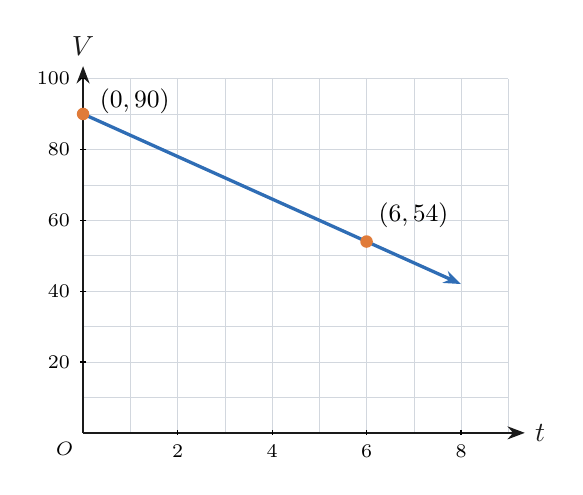
\begin{tikzpicture}[x=0.6cm,y=0.45cm,scale=1.0]
\tikzset{axisline/.style={-{Stealth[length=2.2mm]},thick,INK},gridl/.style={LINE!80,very thin},
 ln/.style={very thick,BLUE},pt/.style={circle,fill=ORANGE,inner sep=1.6pt}}
\draw[gridl] (0,0) grid[xstep=1,ystep=1] (9,10);
\draw[axisline] (0,0) -- (9.35,0) node[right]{$t$};
\draw[axisline] (0,0) -- (0,10.35) node[above]{$V$};
\draw (2,0.07)--(2,-0.07) node[below,font=\scriptsize]{$2$};
\draw (4,0.07)--(4,-0.07) node[below,font=\scriptsize]{$4$};
\draw (6,0.07)--(6,-0.07) node[below,font=\scriptsize]{$6$};
\draw (8,0.07)--(8,-0.07) node[below,font=\scriptsize]{$8$};
\draw (0.07,2)--(-0.07,2) node[left,font=\scriptsize]{$20$};
\draw (0.07,4)--(-0.07,4) node[left,font=\scriptsize]{$40$};
\draw (0.07,6)--(-0.07,6) node[left,font=\scriptsize]{$60$};
\draw (0.07,8)--(-0.07,8) node[left,font=\scriptsize]{$80$};
\draw (0.07,10)--(-0.07,10) node[left,font=\scriptsize]{$100$};
\node[below left,font=\scriptsize] at (0,0) {$O$};
\draw[ln,-{Stealth[length=2.2mm]}] (0,9)--(8,4.2);
\node[pt] at (0,9){};\node[pt] at (6,5.4){};
\node[right,font=\small] at (0.15,9.35) {$(0,90)$};\node[above right,font=\small] at (6.05,5.5) {$(6,54)$};\end{tikzpicture}\end{center}\worklines{6}\end{minipage}\par\vspace{2pt}

\begin{minipage}{\linewidth}\textbf{\textcolor{NAVY}{12.}}\hfill\lvl{Medium \textperiodcentered\ No calculator needed}\\[1pt]For the line $kx+3y=12$ in the $xy$-plane, $k$ is a constant. If the slope of the line is $-2$, what is the value of $k$?\choice{$-6$}{$-2$}{$2$}{$6$}\worklines{6}\end{minipage}\par\vspace{2pt}

\begin{minipage}{\linewidth}\textbf{\textcolor{NAVY}{13.}}\hfill\lvl{Medium \textperiodcentered\ No calculator needed}\\[1pt]A line in the $xy$-plane passes through $(-1,4)$ and $(3,12)$. What is the $y$-coordinate of the point on the line with $x$-coordinate $10$?\worklines{6}\end{minipage}\par\vspace{2pt}

\begin{minipage}{\linewidth}\textbf{\textcolor{NAVY}{14.}}\hfill\lvl{Medium \textperiodcentered\ No calculator needed}\\[1pt]In the $xy$-plane, the line $2x+3y=12$ and the coordinate axes bound a triangle. What is the area of the triangle?\choice{$6$}{$12$}{$24$}{$36$}\worklines{6}\end{minipage}\par\vspace{2pt}

\begin{minipage}{\linewidth}\textbf{\textcolor{NAVY}{15.}}\hfill\lvl{Medium \textperiodcentered\ No calculator needed}\\[1pt]The points $(1,2)$, $(4,8)$, and $(k,20)$ lie on the same line in the $xy$-plane. What is the value of $k$?\worklines{6}\end{minipage}\par\vspace{2pt}

\begin{minipage}{\linewidth}\textbf{\textcolor{NAVY}{16.}}\hfill\lvl{Medium \textperiodcentered\ No calculator needed}\\[1pt]The functions $f$ and $g$ are defined by $f(x)=5x+12$ and $g(x)=2x-9$. The function $h$ is defined by $h(x)=f(x)-g(x)$. What is the $x$-coordinate of the $x$-intercept of the graph of $y=h(x)$?\worklines{6}\end{minipage}\par\vspace{2pt}

\begin{minipage}{\linewidth}\textbf{\textcolor{NAVY}{17.}}\hfill\lvl{Hard \textperiodcentered\ Desmos}\\[1pt]In the $xy$-plane, points $P(-2,1)$ and $Q(6,5)$ are the endpoints of a segment. Which equation represents the perpendicular bisector of $\overline{PQ}$?\choice{$y=\tfrac12x+2$}{$y=-\tfrac12x+4$}{$y=2x-1$}{$y=-2x+7$}\worklines{8}\end{minipage}\par\vspace{2pt}

\begin{minipage}{\linewidth}\textbf{\textcolor{NAVY}{18.}}\hfill\lvl{Hard \textperiodcentered\ Desmos}\\[1pt]In the $xy$-plane, line $\ell$ is shown. Line $m$ is perpendicular to $\ell$ and passes through the $y$-intercept of $\ell$. What is the area of the triangle bounded by $\ell$, $m$, and the $x$-axis?\begin{center}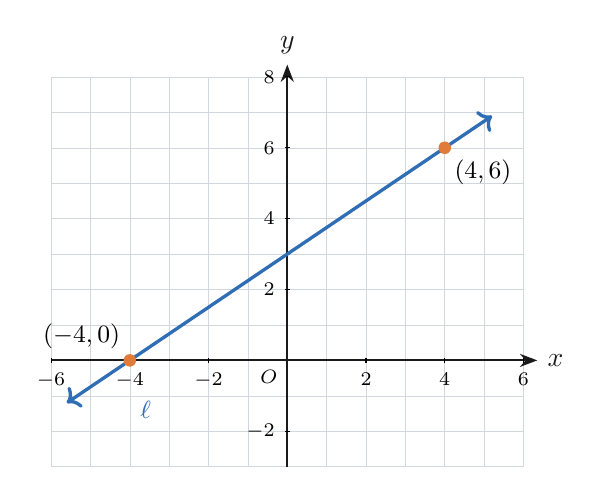
\begin{tikzpicture}[x=0.5cm,y=0.45cm,scale=1.0]
\tikzset{axisline/.style={-{Stealth[length=2.2mm]},thick,INK},gridl/.style={LINE!80,very thin},
 ln/.style={very thick,BLUE},pt/.style={circle,fill=ORANGE,inner sep=1.6pt}}
\draw[gridl] (-6,-3) grid[xstep=1,ystep=1] (6,8);
\draw[axisline] (-6,0) -- (6.35,0) node[right]{$x$};
\draw[axisline] (0,-3) -- (0,8.35) node[above]{$y$};
\draw (-6,0.07)--(-6,-0.07) node[below,font=\scriptsize]{$-6$};
\draw (-4,0.07)--(-4,-0.07) node[below,font=\scriptsize]{$-4$};
\draw (-2,0.07)--(-2,-0.07) node[below,font=\scriptsize]{$-2$};
\draw (2,0.07)--(2,-0.07) node[below,font=\scriptsize]{$2$};
\draw (4,0.07)--(4,-0.07) node[below,font=\scriptsize]{$4$};
\draw (6,0.07)--(6,-0.07) node[below,font=\scriptsize]{$6$};
\draw (0.07,-2)--(-0.07,-2) node[left,font=\scriptsize]{$-2$};
\draw (0.07,2)--(-0.07,2) node[left,font=\scriptsize]{$2$};
\draw (0.07,4)--(-0.07,4) node[left,font=\scriptsize]{$4$};
\draw (0.07,6)--(-0.07,6) node[left,font=\scriptsize]{$6$};
\draw (0.07,8)--(-0.07,8) node[left,font=\scriptsize]{$8$};
\node[below left,font=\scriptsize] at (0,0) {$O$};
\draw[ln,<->] (-5.6,-1.2)--(5.2,6.9);
\node[pt] at (-4,0){};\node[pt] at (4,6){};
\node[above left,font=\small] at (-4,0.05){$(-4,0)$};\node[below right,font=\small] at (4,5.95){$(4,6)$};
\node[BLUE,font=\small] at (-3.6,-1.4){$\ell$};\end{tikzpicture}\end{center}\worklines{8}\end{minipage}\par\vspace{2pt}

\begin{minipage}{\linewidth}\textbf{\textcolor{NAVY}{19.}}\hfill\lvl{Hard \textperiodcentered\ Desmos}\\[1pt]A line in the $xy$-plane passes through $(2,3)$. Its $x$-intercept is twice its $y$-intercept, and neither intercept is $0$. What is the $x$-intercept of the line?\worklines{8}\end{minipage}\par\vspace{2pt}

\begin{minipage}{\linewidth}\textbf{\textcolor{NAVY}{20.}}\hfill\lvl{Hard \textperiodcentered\ No calculator needed}\\[1pt]For a linear function $f$, $f(a+2)-f(a)=6$ for every real number $a$, and $f(0)=-1$. What is $f(5)$?\choice{$11$}{$14$}{$29$}{$30$}\worklines{8}\end{minipage}\par\vspace{2pt}

\begin{minipage}{\linewidth}\textbf{\textcolor{NAVY}{21.}}\hfill\lvl{Hard \textperiodcentered\ Calculator}\\[1pt]Nora's savings grow linearly. On day $3$ she has $250$ SAR and on day $9$ she has $490$ SAR. On what is the first day on which she has at least $1000$ SAR?\worklines{8}\end{minipage}\par\vspace{2pt}

\begin{minipage}{\linewidth}\textbf{\textcolor{NAVY}{22.}}\hfill\lvl{Hard \textperiodcentered\ Desmos}\\[1pt]In the $xy$-plane, the lines $(k+1)x+6y=5$ and $2x+ky=9$ are perpendicular. What is the value of $k$?\worklines{8}\end{minipage}\par\vspace{2pt}

\begin{minipage}{\linewidth}\textbf{\textcolor{NAVY}{23.}}\hfill\lvl{SAT Challenge \textperiodcentered\ Desmos}\\[1pt]In the $xy$-plane, a line with negative slope passes through the point $P(4,3)$ shown. Together with the positive $x$- and $y$-axes it forms a right triangle of area $24$. What is the slope of the line?\begin{center}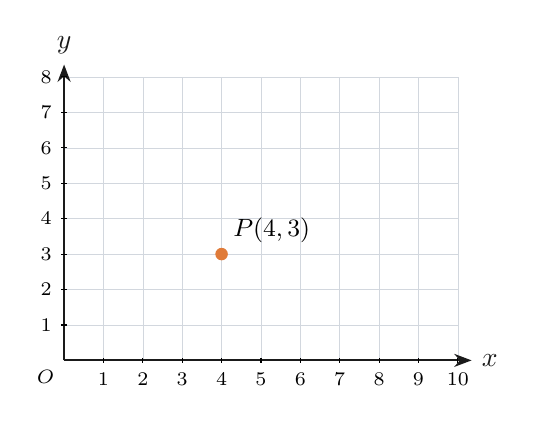
\begin{tikzpicture}[x=0.5cm,y=0.45cm,scale=1.0]
\tikzset{axisline/.style={-{Stealth[length=2.2mm]},thick,INK},gridl/.style={LINE!80,very thin},
 ln/.style={very thick,BLUE},pt/.style={circle,fill=ORANGE,inner sep=1.6pt}}
\draw[gridl] (0,0) grid[xstep=1,ystep=1] (10,8);
\draw[axisline] (0,0) -- (10.35,0) node[right]{$x$};
\draw[axisline] (0,0) -- (0,8.35) node[above]{$y$};
\draw (1,0.07)--(1,-0.07) node[below,font=\scriptsize]{$1$};
\draw (2,0.07)--(2,-0.07) node[below,font=\scriptsize]{$2$};
\draw (3,0.07)--(3,-0.07) node[below,font=\scriptsize]{$3$};
\draw (4,0.07)--(4,-0.07) node[below,font=\scriptsize]{$4$};
\draw (5,0.07)--(5,-0.07) node[below,font=\scriptsize]{$5$};
\draw (6,0.07)--(6,-0.07) node[below,font=\scriptsize]{$6$};
\draw (7,0.07)--(7,-0.07) node[below,font=\scriptsize]{$7$};
\draw (8,0.07)--(8,-0.07) node[below,font=\scriptsize]{$8$};
\draw (9,0.07)--(9,-0.07) node[below,font=\scriptsize]{$9$};
\draw (10,0.07)--(10,-0.07) node[below,font=\scriptsize]{$10$};
\draw (0.07,1)--(-0.07,1) node[left,font=\scriptsize]{$1$};
\draw (0.07,2)--(-0.07,2) node[left,font=\scriptsize]{$2$};
\draw (0.07,3)--(-0.07,3) node[left,font=\scriptsize]{$3$};
\draw (0.07,4)--(-0.07,4) node[left,font=\scriptsize]{$4$};
\draw (0.07,5)--(-0.07,5) node[left,font=\scriptsize]{$5$};
\draw (0.07,6)--(-0.07,6) node[left,font=\scriptsize]{$6$};
\draw (0.07,7)--(-0.07,7) node[left,font=\scriptsize]{$7$};
\draw (0.07,8)--(-0.07,8) node[left,font=\scriptsize]{$8$};
\node[below left,font=\scriptsize] at (0,0) {$O$};
\node[pt] at (4,3){};\node[above right,font=\small] at (4.05,3.05){$P(4,3)$};\end{tikzpicture}\end{center}\worklines{10}\end{minipage}\par\vspace{2pt}

\begin{minipage}{\linewidth}\textbf{\textcolor{NAVY}{24.}}\hfill\lvl{SAT Challenge \textperiodcentered\ No calculator needed}\\[1pt]The linear function $f(x)=ax+b$ satisfies $f(f(x))=9x+8$ for all real $x$. What is the greatest possible value of $f(1)$?\worklines{10}\end{minipage}\par\vspace{2pt}

\newpage\banner{8 \textperiodcentered\ Hint Section \textemdash\ hints only, no solutions}
\begin{enumerate}[leftmargin=1.6em,itemsep=1.5pt,label=\textbf{\arabic*.}]
\item Subtract in the same order on top and bottom.
\item Read the $y$-intercept, then count rise over run to the next lattice point.
\item At an $x$-intercept, $y=0$.
\item Move from $x=3$ to $x=0$: three steps of $-5$.
\item Slope = change in cost per one more session.
\item Same slope; use point-slope with $(1,2)$.
\item Slope of the given line is $-\frac25$; take the negative reciprocal.
\item Get the slope from the two complete columns.
\item Slope $=-\frac{b}{a}$ with $a=-4,\ b=6$; then $y=mx+6$.
\item New equation: subtract $5$ from the right side.
\item Rate $=\frac{\Delta V}{\Delta t}$ between the two labeled points; then solve $V=0$.
\item Solve for $y$, or use $m=-\frac AB$.
\item Slope first; then move $11$ units in $x$ from $x=-1$.
\item Find both intercepts; they are the legs.
\item Equal slopes between any two pairs.
\item Simplify $h(x)$ first; its $x$-intercept is where $h(x)=0$.
\item Midpoint first; then the negative reciprocal of the segment's slope.
\item Read the two labeled points; get $\ell$, then $m$; the $x$-axis chord is the base.
\item If the $y$-intercept is $b$, the $x$-intercept is $2b$; use $\frac{x}{2b}+\frac yb=1$.
\item The difference over an $x$-step of $2$ is $2m$.
\item Model $f(d)$, solve $f(d)\ge1000$, then choose the first whole day.
\item For $A_1x+B_1y=C_1$ and $A_2x+B_2y=C_2$, perpendicular means $A_1A_2+B_1B_2=0$.
\item With intercepts $a,b$: $ab=48$ and $\frac4a+\frac3b=1$. Eliminate one unknown.
\item Expand $f(f(x))$ and match coefficients: two equations, two cases for $a$.
\end{enumerate}
\newpage\banner{9 \textperiodcentered\ Full Solutions}
\begin{minipage}{\linewidth}\textbf{\textcolor{NAVY}{1.}} \textbf{Answer: (A)}.\ $m=\frac{-7-5}{4-(-2)}=\frac{-12}6=-2$.\end{minipage}\par\vspace{5pt}
\begin{minipage}{\linewidth}\textbf{\textcolor{NAVY}{2.}} \textbf{Answer: (C)}.\ $y$-intercept $2$. From $(0,2)$ to $(2,-1)$: rise $-3$, run $2$, so $m=-\frac32$. $y=-\frac32x+2$. (D) reuses $-1$ as the intercept.\end{minipage}\par\vspace{5pt}
\begin{minipage}{\linewidth}\textbf{\textcolor{NAVY}{3.}} \textbf{Answer: (A)}.\ $5x=30\Rightarrow x=6$.\end{minipage}\par\vspace{5pt}
\begin{minipage}{\linewidth}\textbf{\textcolor{NAVY}{4.}} \textbf{Answer: $-8$}.\ $f(0)=7-3(5)=-8$.\end{minipage}\par\vspace{5pt}
\begin{minipage}{\linewidth}\textbf{\textcolor{NAVY}{5.}} \textbf{Answer: (C)}.\ $45$ is the slope: each additional session adds $45$ SAR. ($120$ is the registration fee.)\end{minipage}\par\vspace{5pt}
\begin{minipage}{\linewidth}\textbf{\textcolor{NAVY}{6.}} \textbf{Answer: (B)}.\ $m=3$: $y-2=3(x-1)\Rightarrow y=3x-1$. (A) is perpendicular; (C) is the given line itself; (D) reuses $2$ as the intercept.\end{minipage}\par\vspace{5pt}
\begin{minipage}{\linewidth}\textbf{\textcolor{NAVY}{7.}} \textbf{Answer: $-7$}.\ $m_\perp=\frac52$. $y-3=\frac52(x-4)\Rightarrow y=\frac52x-7$. $y$-intercept: $-7$.\end{minipage}\par\vspace{5pt}
\begin{minipage}{\linewidth}\textbf{\textcolor{NAVY}{8.}} \textbf{Answer: $32$}.\ $m=\frac{20-11}{5-2}=3$. $p=20+3(9-5)=32$.\end{minipage}\par\vspace{5pt}
\begin{minipage}{\linewidth}\textbf{\textcolor{NAVY}{9.}} \textbf{Answer: (C)}.\ $m=\frac{6-0}{0-(-4)}=\frac32$, $y=\frac32x+6$. At $x=2$: $y=9$. So $(2,9)$.\end{minipage}\par\vspace{5pt}
\begin{minipage}{\linewidth}\textbf{\textcolor{NAVY}{10.}} \textbf{Answer: $1$}.\ $y=-2x+2$; set $y=0$: $x=1$.\end{minipage}\par\vspace{5pt}
\begin{minipage}{\linewidth}\textbf{\textcolor{NAVY}{11.}} \textbf{Answer: $15$}.\ $m=\frac{54-90}{6-0}=-6$. $V=90-6t=0\Rightarrow t=15$ minutes.\end{minipage}\par\vspace{5pt}
\begin{minipage}{\linewidth}\textbf{\textcolor{NAVY}{12.}} \textbf{Answer: (D)}.\ $3y=-kx+12\Rightarrow m=-\frac k3=-2\Rightarrow k=6$.\end{minipage}\par\vspace{5pt}
\begin{minipage}{\linewidth}\textbf{\textcolor{NAVY}{13.}} \textbf{Answer: $26$}.\ $m=\frac{12-4}{3+1}=2$. $y=4+2(10-(-1))=26$.\end{minipage}\par\vspace{5pt}
\begin{minipage}{\linewidth}\textbf{\textcolor{NAVY}{14.}} \textbf{Answer: (B)}.\ Intercepts $6$ and $4$. Area $=\frac12(6)(4)=12$.\end{minipage}\par\vspace{5pt}
\begin{minipage}{\linewidth}\textbf{\textcolor{NAVY}{15.}} \textbf{Answer: $10$}.\ $m=\frac{8-2}{4-1}=2$; $\frac{20-2}{k-1}=2\Rightarrow k-1=9\Rightarrow k=10$.\end{minipage}\par\vspace{5pt}
\begin{minipage}{\linewidth}\textbf{\textcolor{NAVY}{16.}} \textbf{Answer: $-7$}.\ $h(x)=3x+21=0\Rightarrow x=-7$.\end{minipage}\par\vspace{5pt}
\begin{minipage}{\linewidth}\textbf{\textcolor{NAVY}{17.}} \textbf{Answer: (D)}.\ Midpoint $(2,3)$; slope of $PQ=\frac{4}{8}=\frac12$; perpendicular slope $-2$. $y=-2x+7$. (A) is line $PQ$; (B) drops the reciprocal; (C) drops the negative.\end{minipage}\par\vspace{5pt}
\begin{minipage}{\linewidth}\textbf{\textcolor{NAVY}{18.}} \textbf{Answer: $\tfrac{75}{8}$}.\ $\ell$: $m=\frac{6-0}{4+4}=\frac34$, $y=\frac34x+3$. $m\perp\ell$ through $(0,3)$: $y=-\frac43x+3$, $x$-intercept $\frac94$. Vertices $(-4,0),(\frac94,0),(0,3)$: base $\frac{25}4$, height $3$; area $=\frac12\cdot\frac{25}4\cdot3=\frac{75}8=9.375$.\end{minipage}\par\vspace{5pt}
\begin{minipage}{\linewidth}\textbf{\textcolor{NAVY}{19.}} \textbf{Answer: $8$}.\ $\frac{2}{2b}+\frac3b=1\Rightarrow\frac4b=1\Rightarrow b=4$. $x$-intercept $=8$. ($y=-\frac12x+4$ passes through $(2,3)$.)\end{minipage}\par\vspace{5pt}
\begin{minipage}{\linewidth}\textbf{\textcolor{NAVY}{20.}} \textbf{Answer: (B)}.\ $2m=6\Rightarrow m=3$, $f(x)=3x-1$, $f(5)=14$. (Not $29$: that uses $m=6$.)\end{minipage}\par\vspace{5pt}
\begin{minipage}{\linewidth}\textbf{\textcolor{NAVY}{21.}} \textbf{Answer: $22$}.\ $m=\frac{490-250}{9-3}=40$; $f(d)=40d+130$. $40d+130\ge1000\Rightarrow d\ge21.75$. First whole day: $22$.\end{minipage}\par\vspace{5pt}
\begin{minipage}{\linewidth}\textbf{\textcolor{NAVY}{22.}} \textbf{Answer: $-\tfrac{1}{4}$}.\ $2(k+1)+6k=0\Rightarrow8k=-2\Rightarrow k=-\frac14$. (Check by slopes: $-\frac{k+1}{6}\cdot\left(-\frac2k\right)=\frac{k+1}{3k}=-1$.)\end{minipage}\par\vspace{5pt}
\begin{minipage}{\linewidth}\textbf{\textcolor{NAVY}{23.}} \textbf{Answer: $-\tfrac{3}{4}$}.\ $\frac4a+\frac3b=1\Rightarrow4b+3a=ab=48$. With $b=\frac{48}a$: $\frac{192}a+3a=48\Rightarrow3a^2-48a+192=0\Rightarrow(a-8)^2=0$, so $a=8$, $b=6$. Slope $=-\frac ba=-\frac34$. (The double root shows $24$ is the \emph{smallest} possible area for a line through $P$.)\end{minipage}\par\vspace{5pt}
\begin{minipage}{\linewidth}\textbf{\textcolor{NAVY}{24.}} \textbf{Answer: $5$}.\ $f(f(x))=a^2x+ab+b$. So $a^2=9$ and $b(a+1)=8$. $a=3\Rightarrow b=2$, $f(1)=5$. $a=-3\Rightarrow b=-4$, $f(1)=-7$. Greatest: $5$.\end{minipage}\par\vspace{5pt}
\end{document}